% CFP: https://discourse.llvm.org/t/cfp-llvm-hpc-workshop-at-sc-25/86391
% At least 5 two-column pages, excluding the bibliography and figures

% Submission: Aug 15, 2025
% Internal deadline: Aug 4, 2025

% Topics:
% 1) The LLVM IR generated by OpenMPIRBuilder can be easily optimized by OpenMPOpt pass (the old flang cannot do it)
% 2) The support of math functions for AMDGPU is done by MLIR code which is also used for GPU-specific optimization for other workloads.
% 3) We can reuse AMD downstream NO_LOOP mode which was written for OpenMP C for Fortran (in progress, but the tests show that it's beneficial)

% Detailed plan for #2 proposal:

% General issues:
% Terminology:
%   array descriptor vs dope vector?
% Default compiler:
%   AOMP Flang/upstream flang?
% Default GPU?
% Are we allowed to present some numbers from microbenchmarks? (i.e. very small code snippets used only for illustration of the problem)

% 1) Handling of descriptors of Fortran pointers and allocatable arrays (The code with allocatable arrays requires more resources in comparison to stack arrays)
%  -> Fortran differences between static and dynamic arrays vs C:
%     a) static -> the size is known in compilation time
%     b) dynamic -> the size and shape is unknown in compilation time
%     c) allocate vs malloc in C
%        * allocate -> defines the shape and size of the allocated array. The information about size/shape and the beginning of allocated memory is stored in array descriptor.
%        * malloc -> allocates N consecutive bytes and it returns address of the first byte
%  -> MLIR(HLFIR + FIR)+LLVM IR code analysis of simple operation a[i] = 5 for static and dynamic arrays for code:
%  !$omp target teams distribute parallel do map(tofrom: x)
%  do i = 1, 255
%    x(i) = a(i) + b(i)
%   end do
%     a) host side + mapping
%     b) GPU side
%  -> Comparison of required resources for exemplary kernels: SGPRS/VGPRS for different optimization levels (are we allowed?)

% 2) Problems related to temporary arrays (i.e.: iaVS = [ iV, jV, kV ] + iaS ) and option -fstack-arrays as remedy.
%  -> Flang default handling of temporary arrays (heap allocation)
%  -> Example of usage of temporary array inside GPU code
%  -> Explanation how heap array is handled inside GPU kernel (slow malloc call)
%  -> Explanation of option -fstack-arrays
%  -> Advantages and disadvantages of option -fstack-arrays (Possible stack overflow vs faster GPU kernels)
%  -> Comparison of execution times for kernel with temporary array with and without -fstack-array (are we allowed?)

%% Lower priority, only as space and time permits:
%% 3) The Fortran runtime calls which can involuntarily appear in the GPU code
%% -> Description of Fortran runtime
%%  -> Examples of Fortran code where Fortran runtime is used
%%  -> Consequences of Fortran runtime call inside GPU kernel (are we allowed to present some execution times?)
\documentclass[acmtog,natbib=false]{acmart}
\AtBeginDocument{\providecommand\BibTeX{{Bib\TeX}}}

\RequirePackage[
datamodel=acmdatamodel,
style=acmnumeric, % use style=acmauthoryear for publications that require it
]{biblatex}
\addbibresource{references.bib}

\usepackage[T1]{fontenc}
\usepackage{listings}
\usepackage{xspace}
\usepackage[printonlyused]{acronym}

% Enabling the next line pushes all figures to the end the paper.
% Michael will occasionally do that to check the page count.
%\usepackage[nomarkers,figuresonly]{endfloat}

%% Rights management information.  This information is sent to you
%% when you complete the rights form.  These commands have SAMPLE
%% values in them; it is your responsibility as an author to replace
%% the commands and values with those provided to you when you
%% complete the rights form.
\setcopyright{acmlicensed}
\copyrightyear{2025}
\acmYear{2025}
\acmDOI{XXXXXXX.XXXXXXX}

%%
%% Submission ID.
%% Use this when submitting an article to a sponsored event. You'll
%% receive a unique submission ID from the organizers
%% of the event, and this ID should be used as the parameter to this command.
\acmSubmissionID{tbd}

%% configure the listings package
\lstset{
  basicstyle=\linespread{0.75}\ttfamily\small,
  captionpos=b,
}

%% useful macros
\newcommand{\todo}[1]{\textcolor{red}{#1}}
\newcommand{\code}[1]{\texttt{#1}\xspace}
\newcommand{\registered}[0]{\textsuperscript{\textregistered}\xspace}
\newcommand{\trademark}[0]{\texttrademark\xspace}

\begin{document}
\title{Implementing OpenMP\registered Offload Support in LLVM Flang}

\author{Dominik Adamski}
\email{dominik.adamski@amd.com}
\orcid{}
\affiliation{%
  \institution{Advanced Micro Devices}
  \city{Lodz}
  \state{lodzkie }
  \country{Poland}
}

\author{Akash Banerjee}
\email{akash.banerjee@amd.com}
\orcid{}
\affiliation{%
  \institution{Advanced Micro Devices}
  \city{Milton Keynes}
  \state{England}
  \country{UK}
}

\author{Kareem Ergawy}
\email{kareem.ergawy@amd.com}
\orcid{0009-0002-6326-8664}
\affiliation{%
  \institution{Advanced Micro Devices GmbH}
  \city{Munich}
  \state{BY}
  \country{Germany}
}

\author{Andrew Gozillon}
\email{andrew.gozillon@amd.com}
\orcid{0000-0001-7558-7166}
\affiliation{%
  \institution{Advanced Micro Devices AB}
  \city{Malmo}
  \state{Skåne County}
  \country{Sweden}
}

\author{Michael Klemm}
\email{michael.klemm@amd.com}
\orcid{0000-0002-8634-4634}
\affiliation{%
  \institution{Advanced Micro Devices GmbH}
  \city{Munich}
  \state{BY}
  \country{Germany}
}

\author{Jan Leyonberg}
\email{jan.leyonberg@amd.com}
\orcid{}
\affiliation{%
  \institution{Advanced Micro Devices}
  \city{Toronto}
  \state{ON}
  \country{Canada}
}

\author{Dan Palermo}
\email{dan.palermo@amd.com}
\orcid{0009-0005-7205-2250}
\affiliation{%
  \institution{Advanced Micro Devices}
  \city{Austin}
  \state{TX}
  \country{USA}
}

\renewcommand{\shortauthors}{Adamski et al.}

\begin{abstract}
\todo{Michael: write the abstract.}
\todo{Lorem ipsum dolor sit amet, consectetur adipisicing elit, sed do eiusmod
tempor incididunt ut labore et dolore magna aliqua. Ut enim ad minim veniam,
quis nostrud exercitation ullamco laboris nisi ut aliquip ex ea commodo
consequat. Duis aute irure dolor in reprehenderit in voluptate velit esse
cillum dolore eu fugiat nulla pariatur. Excepteur sint occaecat cupidatat non
proident, sunt in culpa qui officia deserunt mollit anim id est laborum.
Lorem ipsum dolor sit amet, consectetur adipisicing elit, sed do eiusmod
tempor incididunt ut labore et dolore magna aliqua. Ut enim ad minim veniam,
quis nostrud exercitation ullamco laboris nisi ut aliquip ex ea commodo
consequat. Duis aute irure dolor in reprehenderit in voluptate velit esse
cillum dolore eu fugiat nulla pariatur. Excepteur sint occaecat cupidatat non
proident, sunt in culpa qui officia deserunt mollit anim id est laborum.}
\end{abstract}

%% generate via: https://dl.acm.org/ccs
\begin{CCSXML}
<ccs2012>
   <concept>
       <concept_id>10011007.10011006.10011041</concept_id>
       <concept_desc>Software and its engineering~Compilers</concept_desc>
       <concept_significance>500</concept_significance>
       </concept>
   <concept>
       <concept_id>10010147.10010169.10010175</concept_id>
       <concept_desc>Computing methodologies~Parallel programming languages</concept_desc>
       <concept_significance>500</concept_significance>
       </concept>
   <concept>
       <concept_id>10010520.10010521.10010542.10010546</concept_id>
       <concept_desc>Computer systems organization~Heterogeneous (hybrid) systems</concept_desc>
       <concept_significance>500</concept_significance>
       </concept>
 </ccs2012>
\end{CCSXML}
\ccsdesc[500]{Software and its engineering~Compilers}
\ccsdesc[500]{Computing methodologies~Parallel programming languages}
\ccsdesc[500]{Computer systems organization~Heterogeneous (hybrid) systems}

\keywords{LLVM, Flang, OpenMP, GPU, Accelerators}

\received{20 February 2007}
\received[revised]{12 March 2009}
\received[accepted]{5 June 2009}

\maketitle

%%%%%%%%%%%%%%%%%%%%%%%%%%%%%%%%%%%%%%%%%%%%%%%%%%%%%%%%%%%%%%%%%%%%%%%%%%%%%%%%%%%%%%%%%%%%%%%%%%%%%%%%%%%%
%%%%%%%%%%%%%%%%%%%%%%%%%%%%%%%%%%%%%%%%%%%%%%%%%%%%%%%%%%%%%%%%%%%%%%%%%%%%%%%%%%%%%%%%%%%%%%%%%%%%%%%%%%%%

\section{Introduction}
\label{sec:Introduction}
\todo{Michael: Write the introduction part}

\todo{
\begin{itemize}
\item Fortran standard supported by Flang
\item OpenMP versions supported by Flang
\item Implementations of features driven by request and usefulness, not by historic order.
\end{itemize}
}

%%%%%%%%%%%%%%%%%%%%%%%%%%%%%%%%%%%%%%%%%%%%%%%%%%%%%%%%%%%%%%%%%%%%%%%%%%%%%%%%%%%%%%%%%%%%%%%%%%%%%%%%%%%%
%%%%%%%%%%%%%%%%%%%%%%%%%%%%%%%%%%%%%%%%%%%%%%%%%%%%%%%%%%%%%%%%%%%%%%%%%%%%%%%%%%%%%%%%%%%%%%%%%%%%%%%%%%%%

\section{LLVM Flang Compiler}
\label{sec:LLVMFlangCompiler}

At the time of writing this paper, the AMD Fortran compiler toolchain is undergoing a transition.
AMD is actively working on developing the AMD Next-Gen Fortran compiler that will eventually replace the previously existing AMD Fortran Compiler for the AMD ROCm\trademark platform.
While the current Fortran compiler that ships with AMD ROCm\trademark package is based on the PGI\registered compiler code~\cite{Lara17,Pric17}, the AMD Next-Gen Fortran Compiler is based on the LLVM Flang compiler~\cite{LLVM25}.
AMD plans to make this the new production compiler that will ship with a future version of the AMD ROCm\trademark software stack.

\subsection{Fortran Compiler Pipeline}
\label{sec:FortranCompilerPipeline}

\begin{figure}[t]
\centering
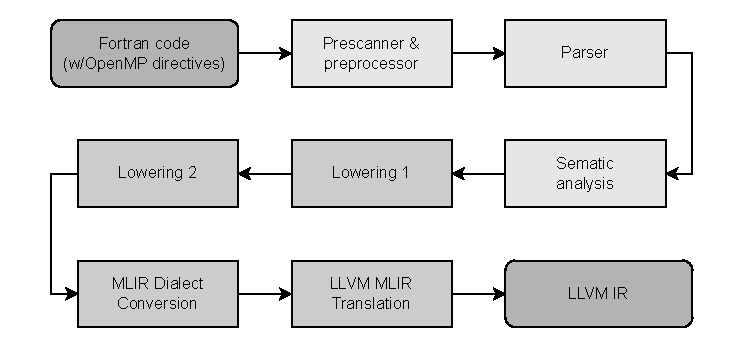
\includegraphics[width=\linewidth]{figures/flang_compiler_phases_overview.pdf}
\caption{Simplified overview of the compiler phases in the AMD Next-Gen Fortran Compiler front-end.\label{fig:FlangCompilerPhases}}
\end{figure}

\begin{figure}[t]
\lstinputlisting[language=Fortran,
                caption={Example Fortran code with \code{!\$omp target team loop} construct and \code{map} clauses},
                label={lst:FortranExample}]
                {code/tgt_loop.f90}
\end{figure}

\begin{figure}[t]
\lstinputlisting[%language=Fortran,
                caption={Fortran code of Listing~\ref{lst:FortranExample} after preprocessing and prescanning.},
                label={lst:FortranExampleCooked}]
                {code/tgt_loop_cooked.f90}
\end{figure}

Figure~\ref{fig:FlangCompilerPhases} shows a simplified overview of the compiler pipeline of the LLVM Flang compiler frontend up to LLVM \ac{IR} generation.
The same stages are also used by the AMD Next-Gen Fortran Compiler front-end.
In the Prescanner \& Preprocessor stage, the lexical analysis and C-style processor produce a stream of characters of normalized Fortran source code. 
This code contains expanded preprocessor macros, included code resulting from \code{INCLUDE} statements, and removed unnecessary blank characters and comments (see Listing~\ref{lst:FortranExampleCooked}).
Compiler directives such as \code{!\$dir} and the OpenMP directives introduced with \code{!\$omp} remain in the stream of characters.
The parser and semantic analysis stages then construct a parse tree of the processed Fortran code and annotate it with semantic information (e.g., data types).
The parse tree contains all details about OpenMP directives, clauses, etc. as nodes in the tree.

\begin{figure}[t]
\lstinputlisting[%language=Fortran,
                caption={Abridged \ac{FIR} code for the Fortran code in Listing~\ref{lst:FortranExample}.},
                label={lst:FortranExampleFIR}]
                {code/tgt_loop_abridged.fir}
\end{figure}

The parse tree is then gradually lowered into different levels of intermediate representation, depending on the needs of the applied transformation and optimization passes.
First, the parse tree and the contained OpenMP directive structure are transformed into \ac{HLFIR} and \ac{FIR}, both of which are based on \ac{MLIR} (see \ac{FIR} code in Listing~\ref{lst:FortranExampleFIR}).
These intermediate representations provide entities that correspond to Fortran language elements.
\Ac{HLFIR} provides additional high-level information over \ac{FIR} about the specific features and semantics of Fortran (e.g., array operations that can be used to optimize Fortran array statements).
It also has additional information in the type system to represent Fortran attributes for (dummy) variables.

OpenMP directives and clauses are reflected in this intermediate representation via an additional \ac{MLIR} dialect.
Through these additional elements, the intermediate representation contains explicit information about  OpenMP directives and clauses in the code as well as their nesting structure.
For instance, \code{DO} loop nest is associated with the corresponding OpenMP \code{target teams loop} construct (see Listing~\ref{lst:FortranExampleFIR}).
Finally, the \ac{MLIR} code is transformed into regular LLVM \ac{IR} and is passed to the compiler back-end for target code generation.


\subsection{OpenMP Code Generation}
\label{sec:OpenMPCodeGen}

During lowering, the compiler outlines OpenMP \code{target} regions and creates kernel functions per region such that the back-end can generate \ac{GPU} code for those in addition to host code.
The original intermediate code is then replaced with boilerplate code to launch the created kernel functions.
This involves generated code to perform data mapping according to the OpenMP semantics and code to invoke the kernel on the GPU via the runtime libraries.

\todo{Andrew: you could write about the actual lowering and code-gen for OpenMP, focus on GPU code-gen and outlining.}

%%%%%%%%%%%%%%%%%%%%%%%%%%%%%%%%%%%%%%%%%%%%%%%%%%%%%%%%%%%%%%%%%%%%%%%%%%%%%%%%%%%%%%%%%%%%%%%%%%%%%%%%%%%%
%%%%%%%%%%%%%%%%%%%%%%%%%%%%%%%%%%%%%%%%%%%%%%%%%%%%%%%%%%%%%%%%%%%%%%%%%%%%%%%%%%%%%%%%%%%%%%%%%%%%%%%%%%%%

\section{Handling the OpenMP Data-Mapping Environment in Flang}

The OpenMP programming model has a complex set of rules governing data movement between host and device, whilst still incomplete Flang has made significant progress in this area.

\todo{Andrew: Insert more. Perhaps mention we support a variety of other map/data environment features (privatization etc), but we'll stick to the "basics" in this section} 

\subsection{The OMP Dialect Map Operation}

\todo{Andrew: Discuss the OMP dialect map operation fields etc. Can perhaps also mention the fact that it has very basic translation rules between dialects, i.e. just transform the types.}

\subsection{From OpenMP Map Clause to the OMP Dialect}

\subsection{Mapping Complex Fortran Types}

\todo{1) declare target mapping 2) descriptor type mapping 2a) assumed shape/size mapping caveats 3) derived (record) type mapping}

%%%%%%%%%%%%%%%%%%%%%%%%%%%%%%%%%%%%%%%%%%%%%%%%%%%%%%%%%%%%%%%%%%%%%%%%%%%%%%%%%%%%%%%%%%%%%%%%%%%%%%%%%%%%
%%%%%%%%%%%%%%%%%%%%%%%%%%%%%%%%%%%%%%%%%%%%%%%%%%%%%%%%%%%%%%%%%%%%%%%%%%%%%%%%%%%%%%%%%%%%%%%%%%%%%%%%%%%%

\section{Conclusions}
\label{sec:Conclusions}

\section*{List of Acronyms}

\begin{acronym}[paper]
\acro{AST}[AST]{Abstract Syntax Tree}
\acro{API}[API]{application programming interface}
\acro{CCD}[CCD]{compute complex die}
\acro{CFD}[CFD]{computational fluid dynamics}
\acro{CU}[CU]{compute unit}
\acro{FIR}[FIR]{Fortran intermediate representation}
\acro{GPU}[GPU]{graphics processing unit}
\acro{HLFIR}[HLFIR]{high-level Fortran intermediate representation}
\acro{HPC}[HPC]{high-performance computing}
\acro{IPO}[IPO]{interprocedural optimization}
\acro{IR}[IR]{intermediate representation}
\acro{LTO}[LTO]{link time optimization}
\acro{MLIR}[MLIR]{multi-level intermediate representation}
\acro{XCD}[XCD]{accelerator complex die}
\acro{WENO}[WENO]{weighted essentially non-oscillatory}
\acro{SDK}[SDK]{software development kit}
\acro{HIP}[HIP]{Heterogeneous-computing Interface for Portability}
\acro{IFA}[IFA]{isolated from above}
\acro{PFT}[PFT]{Pre-FIR Tree}
\acro{RTL}[RTL]{run-time library}
\end{acronym}

%%%%%%%%%%%%%%%%%%%%%%%%%%%%%%%%%%%%%%%%%%%%%%%%%%%%%%%%%%%%%%%%%%%%%%%%%%%%%%%%%%%%%%%%%%%%%%%%%%%%%%%%%%%%
%%%%%%%%%%%%%%%%%%%%%%%%%%%%%%%%%%%%%%%%%%%%%%%%%%%%%%%%%%%%%%%%%%%%%%%%%%%%%%%%%%%%%%%%%%%%%%%%%%%%%%%%%%%%


\section*{Acknowledgments}
Copyright 2025 Advanced Micro Devices, Inc.
AMD, the AMD Arrow logo, Instinct, Radeon, and EPYC, and combinations thereof are trademarks of Advanced Micro Devices, Inc.
Other product names used in this publication are for identification purposes only and may be trademarks of their respective companies.

\printbibliography

\end{document}
